\section{The Hubble Suite}
\label{sec:training_setup}

Our goal in training \textsc{Hubble} is to provide a suite of LLMs suitable for academic study. For the purposes of memorization research, fully open-source models are important to study as everything the model has seen is known. \textsc{Hubble} is fully open-source, and all our models, training code, configuration, checkpoints, datasets, and evaluation code are public, following scientific releases like Pythia \citep{DBLP:conf/icml/BidermanSABOHKP23}, Olmo \citep{groeneveld-etal-2024-olmo}, and others \citep{apertus2024,liu2023llm360fullytransparentopensource}. We choose model and dataset sizes that are manageable for academics with limited computing resources (using \citealp{khandelwal2025k} as a reference).
% Our choice of model and dataset sizes reflect several constraints: training these models must fit within our compute budget, the model and dataset sizes must be manageable for academics with limited computing resources \citep[using][as a reference]{khandelwal2025k}, and these models should be comparable to other open-source language models.
% The core experiment in \textsc{Hubble} consists of 8 models in a $2 \times 2 \times 2$ factorial design where we vary the model size (1B or 8B parameters), data condition (standard or perturbed), and training set size (100B or 500B tokens). 
In terms of scale, the largest pretraining dataset size used for \textsc{Hubble} is 500B tokens, which is roughly 22x and 3.7x the Chinchilla optimal training set size for the 1B and 8B parameter models respectively \citep{10.5555/3600270.3602446_chinchilla}. Compared to Pythia, which was trained on the Pile \citep{gao2020pile800gbdatasetdiverse}, \textsc{Hubble} models are trained on roughly 1.6x more tokens. Compared to commercial LLMs like Llama3 which are trained on 15T tokens \citep{grattafiori2024llama3herdmodels}, there is still a significant gap.

\subsection{Pretraining Data}

%\protect\hfbutton{https://huggingface.co/datasets/allegrolab/dclm-baseline-500b_toks}
\textbf{Base corpus.} Our base pretraining corpus is the baseline dataset introduced in DataComp-LM \citep[\textsc{DCLM};][]{NEURIPS2024_19e4ea30_datacomp}. \textsc{DCLM} is a model-based data filtering pipeline over CommonCrawl which improves model performance over a set of representative tasks. We use their filtered dataset, \verb|dclm-baseline-1.0|,
% and take the first global shard (\texttt{01\_of\_10}) and part of the second global shard (\texttt{02\_of\_10})
as source documents for our tokenization pipeline. Since the \textsc{DCLM} corpus is already deduplicated using Bloom filtering, we do not perform this step again. After decontamination (see below), the documents are tokenized with the OLMo tokenizer \citep[from][]{groeneveld-etal-2024-olmo} which produces a corpus of over 500B tokens. Our smaller 100B corpus is a subset of the 500B corpus, consisting of the first 100B training tokens following GPT-NeoX’s fixed random ordering for shuffling and batching from the entire corpus.
% \hfbutton{https://huggingface.co/allenai/OLMo-1B-0724-hf} \texttt{allenai/OLMo-1B-0724-hf} from

% \textbf{\protect\githubbutton{https://github.com/ameyagodbole/hubble-gpt-neox/tree/decontamination/decontamination} Decontamination}
\textbf{Decontamination.} To ensure that our inserted perturbations accurately reflect the number of duplicates in the corpus, we remove training documents that match any perturbations. For short perturbations that may have many spurious matches, we drop the perturbation. Our two-phase procedure for decontamination is described in Appendix \ref{app:decontamination}. This process removes 7540 training documents (removing less than $0.002\%$ of all documents), and manual inspection confirms high precision. 

\begin{figure}
    \centering
    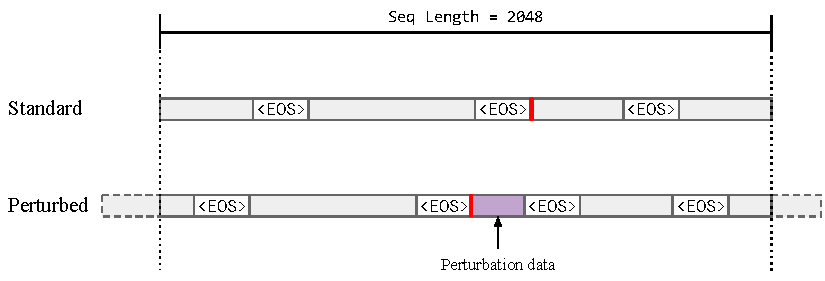
\includegraphics[]{figures/system_diagrams/injection-visualization-v4.pdf}
    \caption{\textbf{Inserting a perturbation.} First, we sample a training sequence from the standard training process to be perturbed. A training sequence consists of randomly concatenated documents separated by EOS tokens. To perturb it, we sample a gap (denoted in red) between the documents and splice the perturbation into a training sequence (between two existing documents). Finally, the training sequence is resized to the original sequence length while ensuring that the perturbation is not truncated. Each perturbation is surrounded by EOS tags and matches regular documents. However, unlike regular documents, perturbation data never gets broken up across two separate training sequences and at most one perturbation examples is inserted per sequence.}
    \label{fig:injection-visualization}
\end{figure}

%\protect\githubbutton{https://github.com/aflah02/tokensmith}
\textbf{Inserting Perturbation Data.} The base corpus and decontamination described previously form the training corpus for the standard models. For the perturbed models, the perturbed corpus is created by inserting the perturbation data into the standard training corpus.\footnote{During our perturbation workflow, we identified the need for a more streamlined setup and consequently developed TokenSmith \citep{khan2025tokensmithstreamliningdataediting}, which consolidates the various scripts we used to edit the tokenized binary files throughout the project. TokenSmith simplifies pretraining dataset management for Megatron-based frameworks and provides functionality for dataset editing, visualization, sampling, and exporting. TokenSmith is available here: \url{https://github.com/aflah02/TokenSmith}.} 
Our insertion attempts to simulate training as if the perturbation was a regular document included in training, and closely matches the order and content of the training sequence in the standard model after perturbation. Figure~\ref{fig:injection-visualization} visualizes an insertion. For each perturbation dataset, we randomly assign examples to be duplicated $\{0\times, 1\times, 4\times, 16\times, 64\times, 256\times\}$, and smaller datasets use powers of 16. To limit the number of examples duplicated 256 times, we assign fewer examples to larger duplication counts  (further details in Appendix~\ref{app:perturbation-data-statistics}).
The perturbations after duplication total to 79.9M tokens (inserted in 818k sequences), which is only 0.08\% of the tokens of the 100B corpus (and 0.016\% for the 500B corpus). Since these duplicates are only a small fraction of the training set, we avoid the issues of \citet{hernandez2022scalinglawsinterpretabilitylearning} who found that language model performance can degrade significantly if there is substantial repeated data in the corpus (more than 3\% in their experiments). We evaluate our models for general capabilities in \S\ref{sec:evaluations} and find no  degradation in the perturbed models. 

\subsection{Models} \label{sec:models}

\textbf{Model architecture.} \textsc{Hubble} models are based off the Llama 3 architecture \citep{touvron2023llamaopenefficientfoundation,grattafiori2024llama3herdmodels}, which we chose due to its popularity. 
A few modifications to this architecture are made for \textsc{Hubble}: first, the smaller OLMo tokenizer is used instead of the original Llama tokenizer (reducing the vocabulary size from 128K to 50K), which substantially reduces the size of the embedding and output projection matrices. The weight embeddings are also untied to support interpretability methods like the logit or tuned lens \cite[consistent with GPT-2 and the Pythia suite studied in][]{nostalgebraist2020logitlens,belrose2025elicitinglatentpredictionstransformers}. Finally, the 8B model has 36 layers instead of 32 in Llama 3.1, to maximize GPU utilization. Appendix \ref{app:training_details} contains more details on our models, considerations, and training setup.

%\wandbbutton{https://api.wandb.ai/links/usc_and_mpi/xzlyob93
\textbf{Runs.} 
% [ANON]The full list of \textsc{Hubble} models are in Appendix \ref{}.
An overview of our models is given below, organized by experiment. The amount of GPU hours consumed for each run is listed in Appendix \ref{app:gpu-hour-logging}.
\begin{itemize}[noitemsep,topsep=0pt]
    \item \textbf{Core.} The core experiment in \textsc{Hubble} formally establishes the phenomenon of dilution, and consists of 8 models in a $2\times2\times2$ factorial design: model size $\{1\text{B}, 8\text{B}\}~\times~$data condition $\{\text{standard}, \text{perturbed}\}~\times~$training set size $\{100\text{B}, 500\text{B}\}$. 

    \item \textbf{Interference.} Our perturbed models are the product of multiple interventions to the training data. To confirm that these interventions minimally interfere with each other, we train three 1B models on 100B tokens with perturbations only in $\{\text{copyright},\text{privacy}, \text{test set contamination} \}$ for comparison against the core perturbed model trained on all perturbations.

    \item \textbf{Timing.} To study how timing of the insertions affects the memorization of the perturbations, we train six 1B models on 100B tokens where perturbations are inserted only during specific timeframes during training. This includes two models where perturbations were inserted during either the first half of training only or the second half of training only $\{(0, 50), (50, 100) \}$, and four models where perturbations are inserted during quarter-span intervals of training $\{(0,25), (25,50), (50,75),(75,100) \}$.

    \item \textbf{Paraphrased.} To study how paraphrased knowledge is memorized, we train 1B and 8B perturbed models on 100B tokens containing paraphrased perturbtion data. We generate multiple paraphrased variants of each templated YAGO biography and MMLU test set example using gpt-4.1-mini. Paraphrasing details are in Appendix \ref{app:paraphrase_results}.

\item \textbf{Architecture.} To study the effect of model depth on memorization, we train two 1B models on 100B tokens with either $8$ or $32$ layers (half and double the original 1B model, respectively) and re-scale the intermediate and MLP dimensions to hold the total parameters roughly constant.
\end{itemize}

%\textbf{Process of Injecting Perturbation in Training Sequences.} A training sequence from the \emph{Standard} corpus consists of concatenated tokens from shuffled documents till the max sequence length. We create the \emph{Perturbed} training sequence by splicing in the tokens of one perturbation document between the documents of the standard training sequence and truncating it to the original sequence length. Thus, no other training sequence is affected/modified. We randomly sample the training sequence (without replacement) and the insertion position for each perturbation.
    
%In the end, because the number of duplicates for each perturbation is randomized and all perturbations are drawn from the same distribution, decontamination does not affect our analyses of the perturbations.


% how did we come up with the buckets?
% 1. Talk briefly of how NeoX is set up
% 2. Talk about ZeRO strategy 
% 3. Tokenizer choice and (potential) changes
% 4. Talk about specific hyperparameters (optimizers, learning rate, etc)
% \todo{Aflah}{Mention where TokenSmith was useful}

%All of our training runs were subject to this compute budget, including 10\% headroom reserved for setup and recovery.

% \todo{Ryan}{Describe how we train, choice of key hyperparams, use of NeoX, any other details needed to replicate results.}
% \textbf{Training configuration}  We train our models using GPT-NeoX \citep{gpt-neox-library}, a pre-training library based on Megatron-LM \citep{megatron-lm} that has been augmented with DeepSpeed and other optimization techniques. For a discussion of the reasons behind this choice and the alternatives considered, refer to Appendix~\ref{app:training-infrastructure-choices}. For all models, we use a global batch size of 1024 with sequence length 2048. We use a learning rate of 4e-4, a minimum learning rate of 4e-5, and a cosine annealing scheduler with a warmup fraction of 0.01 for models trained on 500B tokens and 0.05 for models trained on 100B tokens. We use the Adam optimizer with beta values of 0.9 and 0.95, and an epsilon of 1e-8. We set gradient clipping to 1.0 and weight decay to 0.1. During training, we use stage 1 ZeRO optimization \citep{rajbhandari2020zeromemoryoptimizationstraining}. We accumulate gradients using bf16, but use full precision during allreduce. For more details, please refer to the config file (TO BE ORGANIZED). In total, models trained on 500B tokens experience 238,500 gradient updates, while models trained on 100B tokens experience 48,000 updates.

% \input{tables/main_general_eval}

\subsection{Evaluations} \label{sec:evaluations}

% As part of the \textsc{Hubble} suite, we   the code and results for a base set of evaluations over the model's general performance and memorization.

\textbf{General evaluations.} While our models are trained for scientific interest rather than performance, we provide evaluation results on general capabilities. We evaluate on the same set of tasks as the Pythia suite using the implementations in the Language Model Evaluation Harness \cite[lm-eval-harness;][]{eval-harness}. Table \ref{tab:pythia_general_eval_fewshot} contains the results of our standard models against other open-source and open-weight models. We report additional results and comparisons to models trained on the \textsc{DCLM} corpus in Appendix \ref{app:general_evals}. Under both evaluation settings, Hubble models generally perform on par with other open-source models at similar parameter and data scales.

\textbf{Memorization evaluations.} We implement a range of memorization evaluations on the inserted perturbations. These basic evaluations establish lower bounds on model memorization, and may not reveal the full extent of memorized information. Our evaluations elicit memorization in three ways: 
\begin{enumerate}[noitemsep,topsep=0pt]
    \item \textbf{Loss}. Seen examples can have lower loss compared to unseen examples, and loss can leak membership information \citep{shokri2017membershipinferenceattacksmachine}. Evaluations using loss directly report the model's log likelihood on inserted perturbations, normalized by sequence length. 
    \item \textbf{Loss-based choice}. Many of our inserted perturbations (e.g., test sets) contain alternative answer choices. Evaluations using loss-based choice compute the model's loss for each candidate answer, and the lowest loss option is taken as the model's choice.
    \item \textbf{Generative}. For some perturbations (e.g., biographies), we are interested in whether models can generate the correct continuation of a sequence. Generative evaluation prompts the model to produce a fixed number of next tokens, which are then compared against the ground-truth continuation using exact match or word recall \cite[metrics originally used in][]{rajpurkar-etal-2018-know}.
\end{enumerate}
For the domain-agnostic results in \S\ref{sec:results_domain_agnostic}, the base evaluations we apply for each data type are as follows:
\begin{itemize}[noitemsep,topsep=0pt]
    \item \textbf{Copyright.} For the inserted \textbf{passages} we report loss. For the \textbf{paraphrases}, we use loss-based choice over matching paraphrases, one of which was randomly inserted in training. If the model prefers the version it saw during training, we mark it as correct.

    \item \textbf{Privacy.} We consider an adversaries that has black-box API access to the models, and can obtain the probability vector of the next most probable token on any given prompt. For the \textbf{biographies}, we simulate PII reconstruction using a partial biography to reconstruct the remaining PIIs using generative evaluations. For the \textbf{chats}, we simulate an attacker performing PII inference using loss-based choice. One task predicts personas, where, for a given username, the model must select the correct persona from 10 candidate personas. Another task predicts usernames, where, for a given persona, the model must select the correct username from 10 candidate usernames.

    \item \textbf{Test set contamination.} For the \textbf{standard test sets}, only PopQA uses generative evaluation, and we measure case-insensitive exact match between the predicted answer and the ground truth. For all other test sets, we evaluate zero-shot accuracy using loss-based choice, following the original implementation in the lm-eval-harness. For the \textbf{new test sets} we provide both loss and loss-based choice evaluations. Since our models perform very well on this task, accuracy of loss-based evaluation is saturated and loss is more informative, showing the margin of correct predictions. 
\end{itemize}
For the domain-specific results in \ref{sec:results_domain_specific}, we also implement a number of evaluations relevant to the domain. For copyright we also measure $k$-eidetic memorization on the passages. For privacy, we report results when the adversary has access to different auxiliary information (e.g., predicting an attribute given only the name. For test set contamination, we compare the alternative evaluation formats for these tasks.

% \begin{itemize}[nolistsep]
% \item \textbf{Passages.} The strength of memorization of a passage can be inferred from the (byte-level) perplexity of the language model. To report a metric that is positively correlated, we report the log-likelihood normalized by the sequence length in bytes. Additionally, we measure whether the memorized passages can be easily extracted by prompting the models with the 50-token prefix of passages, and computing the ROUGE-L and exact match scores of the generated continuation.
% \item \textbf{Paraphrases.} We measure whether the language model consistently assigns a high likelihood to one sequence over its paraphrases. We report the accuracy of selecting the injected paraphrase among two choices (the random baseline is 50\% accurate.) We expect models that did not memorize a sequence to have random accuracy in this evaluation. 
%\end{itemize}

% \textbf{Privacy tasks.} This simulates an attacker trying to extract private information given the name (or username in the case of PersonaChat). The format of the prompt depends on the dataset. Additionally, as with the copyright passages, we report the length-normalized log-likelihood of the biography under the model to measure the strength of memorization of the original document.

% \begin{itemize}[nolistsep]
% \item \textbf{Biographies - YAGO.} The synthetic biographies are created with a fixed template. This allows us to clearly identify and group answer entities belonging to each PII type. We create MCQ problems where the model is expected to fill-in-the-blank among 10 choices of the same PII type. We can control the strength of the attack by including more known PII in the prefix and suffix of the MCQ problem. We report the accuracy of the models in predicting the correct PII (a random baseline would achieve 10\% accuracy). We similarly instantiate a generative test where the model is prompted to complete a partial biography (with greedy decoding) instead of being given choices. For the generative evaluation, we report the recall of the answer tokens in the LM's generated response.
% \item \textbf{Biographies - ECtHR.} The biographies of the ECtHR subset are less structured than the YAGO subset. Thus, it is non-trivial to set up multiple-choice evaluations. Thus, we measure whether the LMs can continue a partial biography and generate the PII. Note that earlier PII entities in the original biography will have a shorter prefix and thus be harder to predict than later facts.

% \item \textbf{Chat - PersonaChat.} For this subset, we want to measure whether the LMs can infer indirect information about a person (their persona) through the memorized chat logs. We set up two evaluations: (1) Can the LM correctly associate one out of 10 usernames with the correct persona? (2) Can the LM associate the username with the correct persona out of 10 candidate persons? We choose candidate usernames and personas from within the evaluation set. 
% \end{itemize}

% \textbf{Test set contamination tasks.} For PopQA, we measure the case-insensitive exact match between the predicted answer and the ground-truth answer. For all other test sets, we evaluate zero-shot accuracy.


% \begin{tabularx}{\textwidth}{lccccc}
% \toprule
% Model & Params & Tokens & x & MMLU & y \\
% \midrule
% \multicolumn{6}{l}{\textbf{Open weights, closed datasets}} \\
% \midrule
% Llama2 & 7B & 2T & 49.2 & 45.8 & 34.1 \\
% DeepSeek & 7B & 2T & 50.7 & 48.5 & 35.3 \\
% Mistral-0.3 & 7B & ? & 57.0 & 62.7 & 45.1 \\
% QWEN-2 & 7B & ? & 57.5 & \textbf{71.9} & 50.5 \\
% Llama3 & 8B & 15T & 57.6 & 66.2 & 46.3 \\
% Gemma & 8B & 6T & 57.8 & 64.3 & 44.6 \\
% Phi-3 & 7B & ? & \textbf{61.0} & 69.9 & \textbf{57.9} \\
% \midrule
% \multicolumn{6}{l}{\textbf{Open weights, open datasets}} \\
% \midrule
% Falcon & 7B & 1T & 44.1 & 27.4 & 25.1 \\
% OLMo-1.7 & 7B & 2.1T & 47.0 & 54.0 & 34.2 \\
% MAP-Neo & 7B & 4.5T & \textbf{50.2} & \textbf{57.1} & \textbf{40.4} \\
% \midrule
% \multicolumn{6}{l}{\textbf{Models we trained}} \\
% \midrule
% FineWeb edu & 7B & 0.14T & 38.7 & 26.3 & 22.1 \\
% FineWeb edu & 7B & 0.28T & 41.9 & 37.3 & 24.5 \\
% x & 7B & 0.14T & 44.1 & 38.3 & 25.0 \\
% y & 7B & 0.28T & 48.9 & 50.8 & 31.8 \\
% StarCoder + ProofPile2 & 7B & 2.6T & \textbf{57.1} & \textbf{63.7} & \textbf{45.4} \\
% \bottomrule
% \end{tabularx}



% purpose of the introductory paragraph: situate the reader mentally on what scale of model we are training.

% given our unique computing resource
% hubble is trained in a way to intentionally cause memorization
% its well known duplicates cause memorization \cite{tirumala}
% our perturbations total to less than 0.01% of the data. \cite{hernandaz}
% chinchilla optimal, give a rough idea of the scale of training

% this is roughly 1.5x larger than pythia, but way smaller than llama3
% our dataset is 1TB, which is more researcher friendly.

% The Hubble suite is designed to train realistic language models at a scale suitable for academic study while intentionally inducing memorization on a known set of perturbation data. Our choices for the scale of pre-training corpus, the scale of the models, and the amount of perturbation data are informed by the following considerations: \begin{enumerate}

% \item The total number of models that can be trained (including ablations and testing) is upper bounded by the 200,000 GPU-hour training budget available to us under the NAIRR compute grant. 

% \item We wish to ensure that the Hubble models can be evaluated and fine-tuned on commercially available hardware, facilitating further research. The NVIDIA A100 GPUs, allocated as a part of the NAIRR budget, also set a limit on the model size for efficient training. 

% \item We choose a dataset size of 1TB.

% \item We want to ensure the availability of comparably sized open-source \cite{DBLP:conf/icml/BidermanSABOHKP23,groeneveld-etal-2024-olmo,NEURIPS2024_19e4ea30_datacomp} or open-weight \cite{grattafiori2024llama3herdmodels} models. The open-weight models serve as guidelines and sanity checks for the model quality we can expect for our compute budget.

% \item The total amount of repeated data should comprise a small fraction of the total pre-training data to prevent degradation in model quality \citet{hernandez2022scalinglawsinterpretabilitylearning}.

% \item We want to establish the effect of increasing the size of the pre-training corpus on the memorization of repeated sequences. Unlike prior work, which established the strength of memorization only as a function of the number of duplicates of a sequence \citep{tirumala2022memorization}, we want to study the joint effect of the number of duplicates and the total corpus size. Thus, we want to train the Hubble suite on two different corpus sizes.    \end{enumerate}  

% The Hubble model suite consists of 8 models in a $2 \times 2 \times 2$ factorial design, with the model size $\{1\text{B}, 8\text{B}\} \times$ data condition $\{\text{standard}, \text{perturbed}\} \times$ training set size $\{100\text{B}, 500\text{B}\}$.

% 1B -> 1,179,486,208 params -> 3.73 × 10^21 FLOPs over 500B tokens -> 37.3 / ((1.18)^2 * 1.21)x Chinchilla optimal
% 8B -> 8,265,306,112 params -> 3.1 × 10^22 FLOPs over 500B tokens -> 3.1 / ((8.27/10)^2 * 1.23)x Chinchilla optimal
